%%%%%%%%%%%%%%%%%%%%%%%%%%%%%%%%%%%%%%%%%%%%%%%%%%%%%%%%%%%%%%%%%%%%%%%%%%%
% filename    : main.tex
% author      : 
%%%%%%%%%%%%%%%%%%%%%%%%%%%%%%%%%%%%%%%%%%%%%%%%%%%%%%%%%%%%%%%%%%%%%%%%%%%

% BUGFIX: Save LaTeX kernel version of \@xfloat
\makeatletter
\let\my@xfloat\@xfloat
\makeatother

% use ateneo de naga etd class (actually modified virginia tech's etd class)
\documentclass[oneside]{etd}

% BUGFIX: Create a modified copy of \@xfloat using the kernel definition
\makeatletter
\def\@xfloat#1[#2]{
	\my@xfloat#1[#2]%
	\def\baselinestretch{1}%
	\@normalsize \normalsize
}
\makeatother

% use these packages

\usepackage{graphicx}
\usepackage{amssymb}
\usepackage{gensymb}
\usepackage{latexsym}
\usepackage{amsmath}
%\usepackage[lineno5,noindent]{lgrind}
%\usepackage{rotating} 
%\usepackage{makeidx}
%\usepackage{stmaryrd}
\usepackage{float}
\usepackage{subfigure}
%\usepackage{cite}
%\usepackage{moreverb}
%\usepackage{pictexwd,dcpic}
\usepackage{algorithm,algorithmic}
\renewcommand{\algorithmicrequire}{\textbf{Input:}}
\renewcommand{\algorithmicensure}{\textbf{Output:}}
\usepackage{tikz}
\usetikzlibrary{positioning,calc}

\usepackage{listings}
\definecolor{cppred}{rgb}{0.6,0,0} % for strings
\definecolor{cppgreen}{rgb}{0.25,0.5,0.35} % comments
\definecolor{cpppurple}{rgb}{0.5,0,0.35} % keywords
\definecolor{cppdocblue}{rgb}{0.25,0.35,0.75} % doc
 
\lstset{language=C++,
basicstyle=\linespread{0.8}\ttfamily\small,
keywordstyle=\color{cpppurple}\bfseries,
stringstyle=\color{cppred},
commentstyle=\color{cppgreen},
morecomment=[s][\color{cppdocblue}]{/**}{*/},
numbers=left,
numberstyle=\tiny\color{black},
% stepnumber=2,
numbersep=10pt,
tabsize=4,
showspaces=false,
showstringspaces=false}

\graphicspath{{figures/}{./}}

%\renewcommand{\floatpagefraction}{0.8}

\makeindex

%%%%%%%%%%%%%%%%%%%%%%%%%%%%%%%%%%%%%%%%%%%%%%%%%%%%%%%%%%%%%%%%%%%%%%%%%%%

\title{Synthesis and Evaluation of Amphiphilic Zwitterionic-Fluoropolymer Hybrid Coatings for Non-Biocidal Marine Biofouling Mitigation}
\department{Computer Science}
\BSthesis % options: \BSthesis \BSproject \BShonors \Mdegree \MSdegree \PhDdegree
\degreemonth{December}  % date of final defense
\degreeyear{2026}

\fourstudents % options: \onestudent \twostudents \threestudents \fourstudents
{John A. Doe}
{Jane A. Doe}
{Joe A. Doe}
{Jen A. Doe}

\studentsheader
{Doe, Doe, Doe, Doe}

\fourdegrees % options: \onedegree \twodegrees \threesdegrees \fourdegrees
{Computer Science}
{Computer Science}
{Computer Science}
{Computer Science}

\advisor
{Adviser's Name}
\threemembers
{First Panel Member}
{Second Panel Member}
{Third Panel Member}
\deanandchair
{Dean's Name}
{Chair's Name}

\keywords{firstKeyword, secondKeyword, thirdKeyword}

\begin{document}

%edit etd.cls to accommodate lesser number of proponents
\maketitle
% \makerecomm
% \makeacceptance
% \makedeclaration

%%%%%%%%%%%%%%%%%%%%%%%%%%%%%%%%%%%%%%%%%%%%%%%%%%%%%%%%%%%%%%%%%%%%%%%%%%%
%                    ABSTRACT/EXECUTIVE SUMMARY                           %
%%%%%%%%%%%%%%%%%%%%%%%%%%%%%%%%%%%%%%%%%%%%%%%%%%%%%%%%%%%%%%%%%%%%%%%%%%%

% can use execsummary or abstract
\begin{abstract}
	Marine biofouling on submerged maritime infrastructure incurs substantial economic penalties and operational inefficiencies through hydrodynamic drag and microbially influenced corrosion. While conventional copper-ablative antifouling coatings demonstrate broad biocidal efficacy, their persistent ecotoxicity in benthic sediment layers has driven increasing regulatory restrictions in coastal waters. This thesis investigates the synergistic performance of a non-toxic, amphiphilic zwitterionic-fluoropolymer hybrid coating synthesized via atom transfer radical polymerization (ATRP) on marine-grade structural steel substrates. Using a controlled laboratory flume alongside a six-month field immersion assay in temperate estuarine waters, the synthesized surfaces were evaluated for surface wettability, mechanical shear durability, and settlement deterrence against macro-algal zoospores (Ulva linza) and cyprid larvae of the barnacle Amphibalanus amphitrite. Experimental results indicate that alternating surface charge domains reduced irreversible barnacle cyprid settlement by 84.6\% relative to bare uncoated panels, while contact angle measurements revealed stable surface energetics despite sustained hydrodynamic shear stress exceeding 4.2 Pa. Furthermore, micro-indentation tests confirmed that fluoropolymer domain cross-linking preserved substrate coating adhesion under continuous saline immersion without micro-blistering or delamination. These findings demonstrate that tailored nano-scale amphiphilic topologies offer a viable, environmentally compliant pathway toward non-biocidal marine surface protection, eliminating reliance on heavy-metal leachate mechanisms in littoral zone infrastructure.
\end{abstract}

% \begin{dedication}

We dedicate this research work to all of humanity.

\end{dedication}


% \begin{acknowledgements}

We thank everyone who helped me finish this thesis.

\end{acknowledgements}


\begingroup
\renewcommand*{\addvspace}[1]{}
\tableofcontents
\listoffigures
\listoftables
\endgroup

\beginbody
\pagenumbering{arabic}

%%%%%%%%%%%%%%%%%%%%%%%%%%%%%%%%%%%%%%%%%%%%%%%%%%%%%%%%%%%%%%%%%%%%%%%%%%%
\chapter{Introduction}
%%%%%%%%%%%%%%%%%%%%%%%%%%%%%%%%%%%%%%%%%%%%%%%%%%%%%%%%%%%%%%%%%%%%%%%%%%%
\section{Project Context}

Studies in cognitive load in relation to neurodiversity and their influence in computer science and user experience mostly approach the topic in a qualitative manner, often using methodologies like literature review \cite{burtscher2024, hart2006, kosch2023, liu2024, skulmowski2022, spiel2022, stefanidi2022, wollberg2025, cognitive2025}, interviews \cite{hall2024, lowy2023}, and surveys \cite{conrad2023, robertson2024}. There exist some gaps in the methodologies that aim to quantify and represent cognitive load in HCI researches, especially with neurodivergent participants \cite{lecunff2024}. This study shall implement methodologies that supplement the lack of empirical approaches and potentially invaluable discoveries.

\section{Purpose and Description}

Due to the identified gaps in methodologies and target population of past researches, this study aims to empirically delineate the difference between the cognitive load in neurodivergent and neurotypical population. This study shall utilize the optimal tools and equipment for measuring cognitive load \cite{ahmad2023, appel2019, babu2018, baceviciute2020, hart2006, kosch2023, pretty2024} in these populations, anticipating the potential generation of new insights and knowledge. We shall also discover how the neurodivergent experience differs from the neurotypical experience, understanding the behaviors \cite{hall2024, lowy2023} and strengths \cite{stefanidi2022} of the former in relation to computer studies and systems design. Subsequently, this study will also highlight the lack of inclusivity \cite{lowy2023, wollberg2025} and accessibility \cite{elglaly2024, kuang2024, le2024} to applications and technologies that supposedly cater to neurodivergent populations.

\section{Objectives}

This study aims to:
\begin{itemize}
    \item Get a quantified representation or amount of cognitive load from neurodivergent students in comparison to neurotypical students while using the most common websites.
    \item Understand the experiences of neurodivergent students in relation to HCI and computing by assessing their cognitive load.
    \item Provide a theoretical framework and supporting study for projects that cater to the neurodivergent population.
\end{itemize} 

\section{Scope and Limitations}
This study only aims to look at the cognitive load of neurodivergent and neurotypical students of the same age and education level at the same educational institution. Cognitive stimulation is limited to the use of software to understand the user experience of these user groups. The research will focus on collecting physiological data to monitor the cognitive load of students. The study will not look into the performance of the students while doing various tasks.

\section{Significance}
Understanding the differences of neurotypical and neurodivergent cognitive load under software usage can have a significant impact on future software system designs. This can become a theoretical basis for designing universal and accessible software to allow neurodivergent individuals to benefit from modern software. This study can help fill the gaps of research around the neurodivergent experience \cite{lecunff2024}. The results can serve as a guideline for people involved in software development including the UI/UX Developers, Frontend Developers, and Software Testers.
%%%%%%%%%%%%%%%%%%%%%%%%%%%%%%%%%%%%%%%%%%%%%%%%%%%%%%%%%%%%%%%%%%%%%%%%%%%
\chapter{Review of Related Literature}
%%%%%%%%%%%%%%%%%%%%%%%%%%%%%%%%%%%%%%%%%%%%%%%%%%%%%%%%%%%%%%%%%%%%%%%%%%%

%%%%%%%%%%%%% SECTION 1 %%%%%%%%%%%%%
\section{Cognitive Load Theory}
Cognitive load theory (CLT) studies the strain induced by tasks on human information processing \cite{hart2006, sweller2019architecture}. This theory is based on the assumption that working memory is limited \cite{sweller2010element} and that cognitive overload can reduce performance \cite{howie2023} and learning \cite{sweller2019architecture, klepsch2022}. Experimental data have shown the empirical merits of this theory for understanding human processing of information \cite{ahmad2023} and are applied in the field of education \cite{elglaly2024} and technology \cite{klepsch2022}. Applying this theory to modern technology has shown effectiveness \cite{klepsch2022} and has the potential to create systems that better suit human cognitive architecture.

\subsection{Types of Cognitive Load}
Modern understanding of cognitive load is a three-part model, consisting of intrinsic, extraneous, and  germane cognitive load \cite{sweller1988cognitive, sweller2019architecture, klepsch2022}. Intrinsic cognitive load is load induced by the complexity of information being processed \cite{sweller2019architecture}; this kind of cognitive load is affected both by the information being processed and the expertise of the person receiving the information, since both these factors affect how complex the information being processed is perceived \cite{sweller2019architecture}. A domain expert will have an easier time understanding material in his/her field and thus will have less intrinsic cognitive load. Extraneous cognitive load is another component and is the load induced by the type of medium used to present information \cite{sweller2019architecture}, and other outside factors such noise, comfort and distractions \cite{howie2023}. Different mediums have different effects on cognitive load and can be observed in the split attention effect \cite{sweller2019architecture, thees2020}, and modality effect \cite{sweller2019architecture} of cognitive load research. Germane load is the load associated with schema acquisition or learning \cite{sweller1988cognitive, sweller2019architecture}. Working memory allocated to learning is considered the portion called germane load \cite{sweller2010element}, and is present in cases of moderate cognitive load. Cognitive overload does not allow germane load to occur \cite{sweller2019architecture}, thus little or no schema acquisition happens during cognitive overload.

\subsection{Factors Affecting Cognitive Load}
Experts and novices are differentiated by the amount of schema they have on a particular area of knowledge, not on the amount of working memory they have \cite{hart2006}. The more schema or background knowledge a person has, the more capable they are of solving novel or complex problems in the field by relying on existing strategies for similar problems \cite{hart2006}. Access to long-term memory is infinite, and thus the reliance of existing strategies in long- term memory does not induce high amounts of cognitive resources \cite{hart2006, sweller2019architecture} on experts. In contrast, novices must expend their working memory on new strategies and information to solve problems beyond the capacity of their existing schema on the field \cite{hart2006}. As a result, schema relative to information being processed is a key factor affecting cognitive load. Another factor affecting cognitive load is the medium used to present information \cite{sweller2019architecture}. An example of this factor in practice is how multimedia presentation of information can reduce cognitive load by dividing the loads into different processing segments \cite{sweller2011cognitive}. Using both audio and visual presentation of the same information has been shown to reduce cognitive load by splitting the processing to the visual and auditory segments of human processing \cite{sweller2011cognitive}, instead of overloading a single segment such as visual processing.

\subsection{Cognitive Load Properties}
\subsubsection{Goal-Free Effect}
The goal-free effect states that less cognitive load is received when there’s no specific goal \cite{sweller2019cognitive}. Means-ends analysis is the most generic strategy for solving unfamiliar problems, but it is highly inefficient \cite{hart2006}. Continuously holding in working memory the current state, the goal state, the difference between the two and the legal operations for solving a problem induces a high cognitive load \cite{hart2006}. Without a specific goal in mind, a person is able to perform a similar activity with less cognitive load compared to a person implementing a means-ends strategy. The goal free effect can contribute to learning because cognitive overload could be lessened to allow for schema acquisition.

\subsubsection{Modality Effect}
The modality effect considers the theory that working memory is divided into different sections, such as for visual and auditory \cite{sweller2019cognitive, sweller2011cognitive}. By distributing information into these sections, one is less likely to induce cognitive overload. Cognitive load has been shown to be reduced when presented with the same information when split into audio and visual format compared to only a visual presentation \cite{sweller2011cognitive}.

\subsubsection{Split Attention Effect}
The split-attention effect explains how increased cognitive load is present when a person integrates two sources of information \cite{sweller2019cognitive}. Extraneous cognitive load has been shown to be reduced for those using augmented reality (AR) aids in a physics undergraduate course \cite{klepsch2022}, as information is consolidated realtime using AR technology. 

\subsection{Measuring Cognitive Load}
\subsubsection{Questionnaires}
One methodology in HCI researches is by utilizing questionnaires \cite{hall2024, castanheira2021, ayres2021}. Questionnaires enable subjective responses from the participants, providing HCI studies an overview of the participant and description of experiences and challenges. One famous subjective measure is the NASA-TLX \cite{hall2024, ayres2021} which is famously used in subjective HCI research methodologies to assess mental workload for the above-mentioned aspects. A research instrument such as questionnaires is easily deployable, but it requires extensive use in order to synthesize highly valuable information \cite{castanheira2021}.

\subsubsection{Physiological Measures}
Physiological measures have been shown to be accurate and empirical metrics of cognitive load \cite{lecunff2024, castanheira2021, thees2020}. Eye metrics such as pupil dilation and blink patterns have been shown to be the most sensitive physiological measure to cognitive stimulation \cite{souchet2022, castro-alonso2020modality}. Additionally, other physiological measures of cognitive load exist, such as cerebral \cite{appel2019, babu2018} and cardiovascular \cite{ahmad2023, lecunff2024} measures. These measures provide more insights regarding cognitive load by looking into the physiological reactions of the participants in response to various stimuli and mental tasks. However, compared to questionnaires, physiological measures and instruments are less accessible and difficult to deploy.

\subsection{An Evolving Field of Study}
The cognitive load theory has been applied in various contexts having a common goal: to understand the cognitive effects of the immediate study \cite{sweller2019architecture}. Since its inception, various methods have been implemented and integrated to understand the effects of cognitive load in the performance of human participants in different working tasks \cite{sweller2019architecture}. It is expected that there will be more advancements, and more studies will be conducted that uses the cognitive load theory as their core theoretical framework \cite{sweller2019architecture}.

%%%%%%%%%%%%% SECTION 2 %%%%%%%%%%%%%
\section{Neurodiversity}
Neurodiversity is understood as having different cognitive processes in contrast to neurotypical individuals. It highlights the individual differences in the way that each brain works, and that there is no “correct” way how individuals should think \cite{mack2022, cognitive2025}. In this section, we shall delineate and contextualize neurodiversity in relation to cognitive load, HCI, and computer science.

\subsection{Contextualizing Neurodiversity}
In HCI and computer science, neurodiversity studies frequently look into the subjective aspect, which includes the solicitation of experience and insights from neurodivergent individuals in different settings like school \cite{burtscher2024, cognitive2025} or the workplace \cite{bowman2023, biondi2020, liu2024}. These studies help us understand their unique experiences, preferences, and strengths. With that, this study became more motivated to bridge the gap between empirical methodologies and neurodivergent experiences. Furthermore, the studies also showed us a trend where neurodivergent individuals are often kept from participating in the development of systems and applications that are supposedly dedicated to them \cite{bowman2023, kuang2024, lowy2023, skulmowski2022, spiel2022}, raising a concern in the inclusivity and reliability of the outputs. Consequently, the neurodivergent population, in relation to HCI research, expresses their preference to be part of technological developments \cite{kuang2024, liu2024, skulmowski2022}, providing more valuable insights in the pursuit of a more inclusive technological community. 

\subsection{Neurodiversity and Cognitive Load}
Based on the previous subsections, cognitive load and neurodiversity research, respectively, are plenty. However, studies that delve into the relationship between cognitive load and neurodiversity and their dynamics are highly scarce \cite{vilotijevic2022}, especially how cognitive load plays when neurodiversity is used as an independent variable. A similar study \cite{vilotijevic2022} focusing on the relationship between cognitive load in neurodivergent individuals has discovered and concluded the immense lack of study of those variables through their systematic narrative synthesis. This reinforces the need and impact of a similar study, ensuring an invaluable contribution to the field.

\section{Identified Gaps in Literature and Systems}
There is a lack of study in the area of cognitive load research for neurodivergent individuals  \cite{vilotijevic2022, bowman2023, biondi2020, liu2024}. Research on this area of study could provide opportunities to better serve the population of neurodivergent users in the software industry, as there is a gap in the quality of software for the needs of neurodivergent individuals.

\section{Justification for the Proposal}
The potential of the results of this research will have widespread impact on designing systems for neurodivergent individuals and the general population of software users. The findings of this study could become a basis for designing new conventions and standards for accessible \cite{conrad2023, kosch2023, lowy2023} software design and implementation. Lastly, this research could explore the differences in neurodivergent cognitive processing in relation to the neurotypical, and provide precedence for future research in this largely unexplored area.
%%%%%%%%%%%%%%%%%%%%%%%%%%%%%%%%%%%%%%%%%%%%%%%%%%%%%%%%%%%%%%%%%%%%%%%%%%%
\chapter{Theoretical Framework} 
%may be changed into a Technical Background
%%%%%%%%%%%%%%%%%%%%%%%%%%%%%%%%%%%%%%%%%%%%%%%%%%%%%%%%%%%%%%%%%%%%%%%%%%%

\section{Cognitive Load Theory}
Cognitive load theory (CLT) provides a framework for understanding human cognitive strain and classifies cognitive load into 3 main categories: intrinsic, extraneous, and germane \cite{sweller2019architecture}. Each of these are defined below:
\begin{itemize}
    \item Intrinsic cognitive load is the load induced by the task itself. Intrinsic cognitive load is only affected by two factors: the person and the activity itself. A person’s experience is a key factor in the difficulty induced by a task, because an expert in a task, someone with prior experience with the task or a similar task, receives less cognitive load than a novice, a person with no experience, doing the same task. The difficulty of the task itself affects intrinsic cognitive load, with more difficult tasks increasing cognitive load for the same participant.
\end{itemize}
\begin{itemize}
    \item Extraneous cognitive load is the load induced by the format of information and the environment. Different ways of presenting information induce different cognitive loads. A primary example of this is how visual and auditory media (video) induce lower cognitive load than visual presentation of information alone, a case of the modality effect. The environment also contributes to extraneous cognitive load, where additional stimulation such as noise or discomfort increases cognitive load.
\end{itemize}
\begin{itemize}
    \item Germane cognitive load is the cognitive load spent on learning. Low to moderate cognitive load allows for germane load to occur, whereas cognitive overload does not allow allocation of cognitive resources to allow for learning.
\end{itemize}
These three categories underpin a framework for understanding the factors affecting human cognitive strain. By developing an understanding of human cognitive load during activities, managing cognitive load becomes feasible. As technology and software integrate into the daily lives of people, understanding the implications of using these tools becomes increasingly important. Cognitive load theory can provide a theoretical approach for evaluating human experience while using technology. In this study, CTL will help the researchers identify the effect of different contemporary systems on the cognitive load of neurodivergent and neurotypical users, particularly the intrinsic and extraneous cognitive load associated with the use of software systems themselves.


\section{Pupillometry}
Pupil dilation has been used as a metric for cognitive load in recent years \cite{souchet2022, vilotijevic2022, castanheira2021}. Increased cognitive strain correlates with the dilation of pupils and can be used to map periods of heightened cognitive load, and this approach can be a reliable quantitative metric for evaluating cognitive load. There are other factors that affect pupil size, such as pupil light response, and these generally start at 200 ms, while the onset of task-evoked pupil dilation, such as those in this research, tends to be slow-paced; researchers should observe 2–3 seconds after the onset of stimulation for pupil response \cite{mathot2022}.

\section{Neurodiversity Theory}
Neurodiversity is a cognitive condition that uniquely characterizes an individual’s way of thinking \cite{baumer2021, childmind2025}. This theory highlights the natural variation of the human factor in HCI studies. It must be established that neurodiversity is associated with a unique cognitive ability rather than a deficit \cite{aldersonday2023}, because there exists a trend wherein neurodivergent individuals are kept from co-producing tools and systems that are dedicated to them \cite{burtscher2024, le2024, baumer2021, spiel2022, stefanidi2022}. However, the reason behind why it happens is unknown. Therefore, examining the impacts of neurodiversity on the development of tools, applications, and systems can help create a framework that defines effective approaches and practices grounded in this theory. 
 

\section{Integration of CLT and Neurodiversity}
The interconnection of CLT and neurodiversity is an extremely under-examined area \cite{lecunff2024}. Currently, there is a noticeable lack of frameworks that describe the relationship between these domains, especially in the context of HCI, user experience, and systems design. This extremely novel area of study creates an opportunity for invaluable discoveries and syntheses. This study contributes to the field by proposing a framework that integrates the core concepts of CLT and neurodiversity in relation to the above-mentioned domains. By grounding the framework in both empirical and theoretical findings, this study can establish foundational best practices for future research, development, and implementation of accessible digital tools and environments.

%%%%%%%%%%%%%%%%%%%%%%%%%%%%%%%%%%%%%%%%%%%%%%%%%%%%%%%%%%%%%%%%%%%%%%%%%%%
\chapter{Methodology}
%%%%%%%%%%%%%%%%%%%%%%%%%%%%%%%%%%%%%%%%%%%%%%%%%%%%%%%%%%%%%%%%%%%%%%%%%%%

\section{Sampling}
The participants of this study are students in Saint Joseph School at Naga City, Camarines Sur, Philippines. The study will employ random sampling for selecting neurodivergent participants from the special education classes of Saint Joseph School as the experimental group. A random sample of neurotypical participants as the control group will be selected from the regular classes. Both groups will consist of 6th grade students.

\section{Data Collection}
This study will employ a hybrid method, using a physiological measure through an IoT device for quantitative data (pupil dilation) and an in-person interview to solicit comments and understand the experience of the participants. The participants will be asked to perform tasks using the three most common web applications (Google, YouTube, and Facebook \cite{kemp2025}) while the IoT device measures their pupil size. Additionally, the study will be conducted during the morning in a controlled setting to minimize extraneous cognitive load not relevant to the use of the software system. In particular, the most relevant factors to be controlled in a pupillometry experiment include screen brightness, room brightness, eye position, and outside noise. The software system will be presented to participants, and one by one, tasks will be provided written on a paper. The participants will be asked to wait 2 seconds after being administered the task and will then be allowed to perform the task on the software system. This is to observe the cognitive load induced by both the task and performing the task. 

\section{Data Analysis}
Data visualization will be done using Python and matplotlib to process and represent the quantitative data. The data gathered from the neurodivergent individuals will be compared with the data from the neurotypical individuals, emphasizing whether there is a significant difference between their cognitive loads. Further analysis of the effects of tasks with the software systems will be done using cross-validation for pupillometry experiments \cite{mathot2022}. Moreover, the qualitative responses will be collected and organized through thematic analysis \cite{rosala2022, bowman2023}, reflecting the recurring trends among the participants, as well as valuable insights, comments, and potential complaints.

\begin{figure}
    \centering
    \includegraphics[width=0.75\linewidth]{Manuscript//figures/result-gavsgreedy.pdf}
    \caption{Enter Caption}
    \label{fig:placeholder}
\end{figure}


This is the figure \ref{fig:placeholder}


\begin{table}
    \centering
    \begin{tabular}{ccc}
         &  & \\
         &  & \\
    \end{tabular}
    \caption{Caption}
    \label{tab:placeholder}
\end{table}
% %%%%%%%%%%%%%%%%%%%%%%%%%%%%%%%%%%%%%%%%%%%%%%%%%%%%%%%%%%%%%%%%%%%%%%%%%%%
\chapter{Results and Discussion}
%%%%%%%%%%%%%%%%%%%%%%%%%%%%%%%%%%%%%%%%%%%%%%%%%%%%%%%%%%%%%%%%%%%%%%%%%%%

The researcher conducted an experiment to validate the results
in \cite{Zaritsky2004}'s work. Following is the description of the 
experiment done.

The input strings used in the experiment were generated in a
 manner similar to the one used in DNA sequencing. That is, a random
string is generated, duplicated a predetermined number of times,
 and the copies are randomly divided into blocks of a given size. 
 The set of all these blocks is the input to the SCS problem. 
 The reasons for choosing this type of input has been extensively
 explained in \cite{Zaritsky2004}.
Since our random string is a sequence of characters \texttt{A},\texttt{C},\texttt{G}, and \texttt{T}, we must 
transform this into an equivalent binary string. To do this, we simply 
assign each letter a unique two-bit representation, that is, 
\texttt{A = 00}, \texttt{C = 01}, \texttt{G = 11}, and \texttt{T = 10}. 

The parameters used in the input generation is as follows:

\begin{tabular}{p{0.5cm}l}
&\textit{Size of random string}: 250 bases or characters\\
&\textit{Minimal block size}: 20 characters\\
&\textit{Maximal block size}: 30 characters\\
&\textit{Number of duplicates created from the random string}: 5\\
\end{tabular}

Let $l$ denote the length of the derived string in the
genetic algorithm case. Let $m$
denote the number of blocks not covered by the derived string, 
and let $b$ denote the maximal block size
(30, in our case). The fitness value, $f$ , of an individual
is computed as follows:
\[f = \dfrac{1}{l + m*b}\] 
This fitness function above drives evolution towards
shorter superstrings covering as many blocks as possible.

We performed 50 randomly generated problem instances.
On each problem instance each type of genetic algorithm was executed
twice and the better run of the two was used for statistical purpose.
The results are summarized in Table \ref{tbl:resultsga} and is presented graphically in Figure \ref{fig-results}.


\begin{table}
\centering
\caption{
Average superstring length and runtime of our Genetic Algorithm
on 50 randomly generated problem instances. Each input set contains
50 blocks.}
\label{tbl:resultsga}
\begin{tabular}{|c|c|c|}
\hline
Number  & Average Superstring  & Average  \\
 of& Length (Rounded to & Runtime \\
Generations& Nearest Units) & (in Seconds) \\
\hline
\hline
100		& 760	& 34.57		\\
250		& 596	& 74.20		\\
500		& 526	& 139.70	\\
1000	& 482	& 267.09	\\
5000	& 421	& 1038.73	\\
10000	& 413	& 1943.55	\\
20000	& 409	& 3700.57	\\
\hline
\end{tabular}
\end{table}


\begin{figure*}[ht!]
\centering
\fbox{
\scalebox{0.55}{
\includegraphics{result-gavsgreedy.pdf}
}}
\caption{Best superstring as a function of generations. Each point in the figure represents the average of 50
runs on 50 different randomly generated problem instances. For each such instance, two runs were performed, the better
of which was considered for statistical purposes}
\label{fig-results}
\end{figure*}

Note that our results seem to disagree with that of \cite{Zaritsky2004}.
In contrast with the latter's findings, our tests shows that
the greedy algorithm outperformed the genetic algorithm both in terms of finding superstrings
with minimal length and the the time it takes to do so.

On the same set of test cases, the greedy algorithm
produced superstrings having an average of 361 characters, 
in an average of runtime 130.64 milliseconds. This is far better than
the 409 average superstring length that the genetic algorithm
derived in 20000 generations in more or less an hour of operation. 
Note that the average length of the superstring derived by the greedy algorithm is
less than the conjectured factor-2 performance guarantee.
Recall that the length of the initial (reference) string is 250.

Still it is good to note that the genetic algorithm approach
in solving the SCS problem converges. That is, we see a better solution
yield as time or generations progress. 
% %%%%%%%%%%%%%%%%%%%%%%%%%%%%%%%%%%%%%%%%%%%%%%%%%%%%%%%%%%%%%%%%%%%%%%%%%%%
\chapter{Contributions and Recommendations}
%%%%%%%%%%%%%%%%%%%%%%%%%%%%%%%%%%%%%%%%%%%%%%%%%%%%%%%%%%%%%%%%%%%%%%%%%%%

\section{Summary of Contributions}

Write summary of contributions here.

\section{Recommendations}


There could be several reasons why our tests did not yield the ``same'' results as that of \cite{Zaritsky2004}'s.
The author claims that this may be due to the myriad of parameters used in evolving
individuals in each step of the genetic algorithm and the large number of possible candidates or values that we can set these parameters with. 
For example, we may claim that the appropriate choice of the recombination technique is necessary. In \cite{Zaritsky2004},
a two-point crossover was employed. Thinking that this may be less of a factor, the author proceeded with just
one-point cross in implementing the genetic algorithm for the experiment.
Another could be in choice of the probabilities associated with recombination, elitism, and mutation rates.
The author did only consider what was stated in the base paper without performing tests to validate
whether this values are appropriate and could still complement the change made in some of the assumptions.
As such, more empirical tests could be done to appropriately estimate these parameters. 

If indeed DNA sequence assembly is the task at hand, lots of other techniques are now available.
One may consider for example representing the reads or DNA fragments in a de Bruijn graph
as opposed to the overlap graph presented in this paper. 
Assembling reads  in a de Bruijn graph 
reduces the problem to a fragment assembly problem that can be 
formulated as the goal to find a trail or Eularian path that visits 
each edge (read or fragment) in the (de Bruijn) graph exactly once. 
Such, somehow makes the assembly process much ``easier'' since Eularian path
construction is known to be solvable in deterministic polynomial time.


% %%%%%%%%%%%%%%%%%%%%%%%%%%%%%%%%%%%%%%%%%%%%%%%%%%%%%%%%%%%%%%%%%%%%%%%%%%%
\chapter{Conclusion}
%%%%%%%%%%%%%%%%%%%%%%%%%%%%%%%%%%%%%%%%%%%%%%%%%%%%%%%%%%%%%%%%%%%%%%%%%%%

The SCS problem is NP-Complete but is approximable.
DNA sequence assembly can be approached as an SCS problem by representing
reads or sequence fragments in an overlap graph.
The greedy algorithm in finding an approximate solution to the SCS problem
is simple and has a constant performance guarantee. Our result shows, 
the greedy algorithm was successful in deriving superstrings with 
an average length less than the conjectured factor-2 performance guarantee.
A genetic algorithm is also viable alternative to the greedy approach,
however, as our results have shown, the complexity in terms of defining and estimating
appropriate parameters and the time it would take for one to extract satisfactory solution, 
may be a great hindrance in the practical use of the technique
such as in DNA sequence assembly.
As a proof of concept, we have shown that indeed the genetic algorithm approach
in solving the SCS problem converges. That is, a better solution
is yield as time or the number of generations is increased. 

\appendix
   % Appendix A

\chapter{Appendix Title Here} % Main appendix title
\label{AppendixA} % For referencing this appendix elsewhere, use \ref{AppendixA}

\lhead{Appendix A. \emph{Appendix Title Here}} % This is for the header on each page - perhaps a shortened title

Write your Appendix content here.
   \chapter{Evaluation Tool}

Evaluation tool used goes here.

%    \chapter{Sample Reports}

Describe and discuss the details of sample reports here.

%    \chapter{Sample Input/Output}

Describe and discuss the details of sample I/O here.

%    \chapter{Code Listing}

\lstinputlisting{src/scs-greedy.cpp}

%    \chapter{User's Guide}




\nocite{*}
\bibliographystyle{siam}
{
\singlespace
\bibliography{references}
}

% \begin{vita}

Juan N. Dela Cruz is BS Information Technology student of the Department of Computer Science at the Ateneo de Naga University.
\\
\\
Peter P. San Pedro is BS Information Technology student of the Department of Computer Science at the Ateneo de Naga University.
\\
\\
John J. San Juan is BS Information Technology student of the Department of Computer Science at the Ateneo de Naga University.
\\
\\
Maria Theresa F. Ni\~{n}o is BS Information Technology student of the Department of Computer Science at the Ateneo de Naga University.

\end{vita}

\end{document}
